\section{Neutrino mass ordering sensitivity}
\label{sec:mh_sens}

In this section, the toy throwing approach described in Section~\ref{sec:analysis_framework} is used to explore the neutrino mass ordering sensitivity as a function of exposure in detail.

\begin{figure}[htbp]
  \centering
  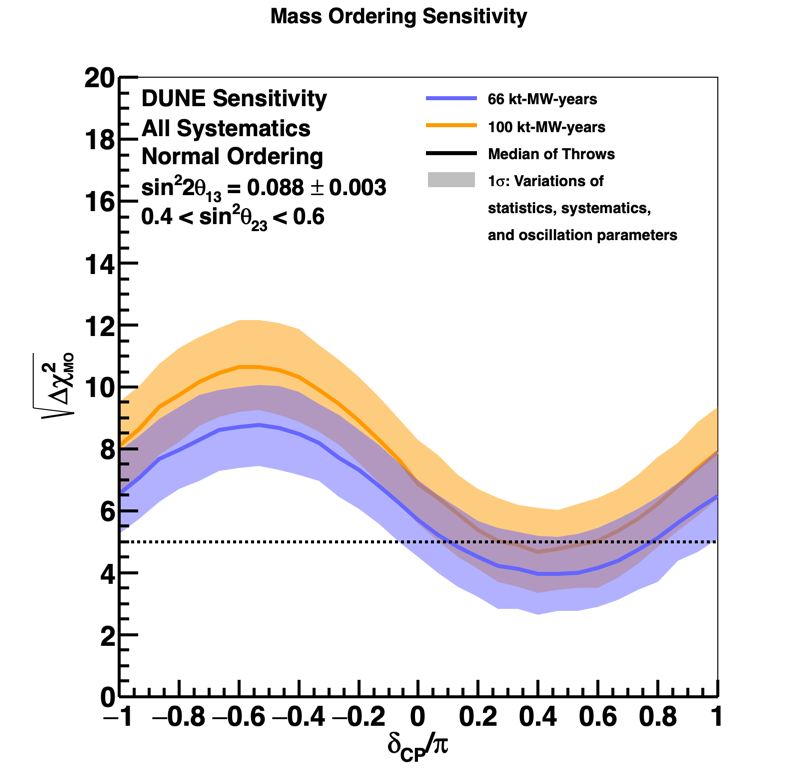
\includegraphics[width=0.8\linewidth, trim={0cm 0cm 0cm 2.3cm}, clip]{mh_two_exps_throws_nh_2019_v4_lowexp.png}
  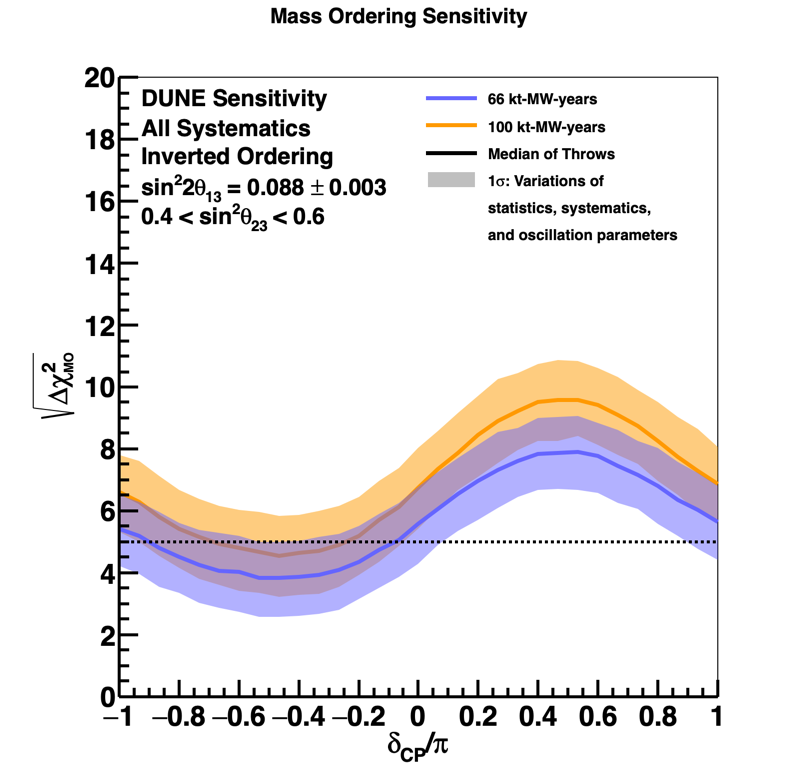
\includegraphics[width=0.8\linewidth, trim={0cm 0cm 0cm 2.3cm}, clip]{mh_two_exps_throws_ih_2019_v4_lowexp.png}
  \caption{Significance of the DUNE determination of the neutrino mass ordering, as a function of the true value of \deltacp, for 66 ktMWyr (blue) and 100 ktMWyr (orange) exposures. The width of the transparent bands cover 68\% of fits in which random throws are used to simulate systematic, oscillation parameter and statistical variations, with independent fits performed for each throw constrained by pre-fit uncertainties. The solid lines show the median sensitivity.}
  \label{fig:mh_bands}
\end{figure}
Figure~\ref{fig:mh_bands} shows the significance with which the neutrino mass ordering can be observed for both true NO and IO, for exposures of 66 kTMWyr and 100 ktMWyr. For each throw of the systematic, other oscillation parameters and statistics, two fits are carried out, one using each ordering. The difference in the best-fit $\chi^{2}$ values is calculated:
\begin{equation}
  \Delta\chi^{2} = \chi^{2}_{\mathrm{IO}} - \chi^{2}_{\mathrm{NO}},
  \label{eq:mh_chi2}
\end{equation}
\noindent and the square root of the difference is used as the figure of merit on the y-axis of Figure~\ref{fig:mh_bands}.

The characteristic shape of the MH sensitivity in Figure~\ref{fig:mh_bands} results from near degeneracy between matter and CPV effects that occurs near $\deltacp=\pi/2$ ($-\deltacp=\pi/2$) for true normal (inverted) ordering. We note that dedicated studies have shown that special attention must be paid to the statistical interpretation of neutrino mass ordering sensitivities~\cite{Ciuffoli:2013rza,Qian:2012zn,Blennow:2013oma} because the \dchisq metric does not follow the expected chi-square function for one degree of freedom, so the interpretation of the $\sqrt{\dchisq}$ as the sensitivity is complicated.

\begin{figure*}[htbp]
  \centering
  \subfloat[6 ktMWyr]   {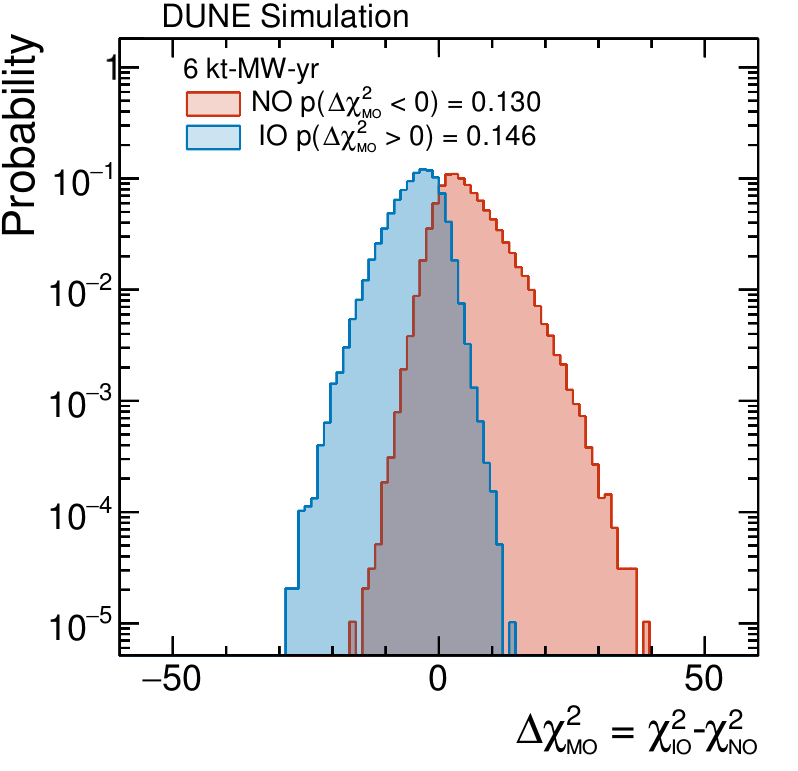
\includegraphics[width=0.33\linewidth]{MH_comp_ndfd_6ktMWyr_th13.png}}
  \subfloat[12 ktMWyr]  {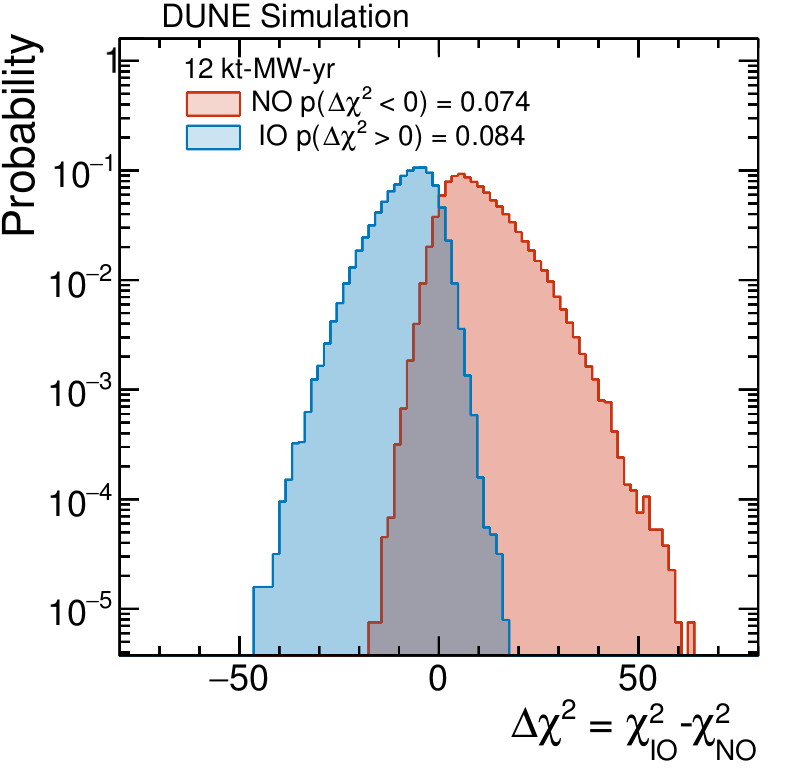
\includegraphics[width=0.33\linewidth]{MH_comp_ndfd_12ktMWyr_th13.png}}
  \subfloat[24 ktMWyr]  {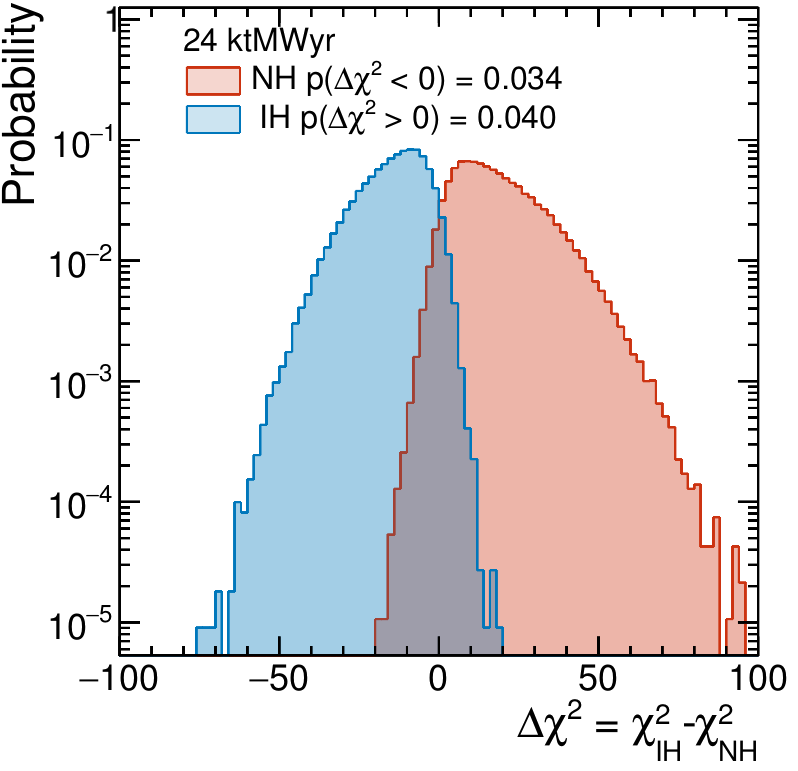
\includegraphics[width=0.33\linewidth]{MH_comp_ndfd_24ktMWyr_th13.png}}\\
  \subfloat[66 ktMWyr]  {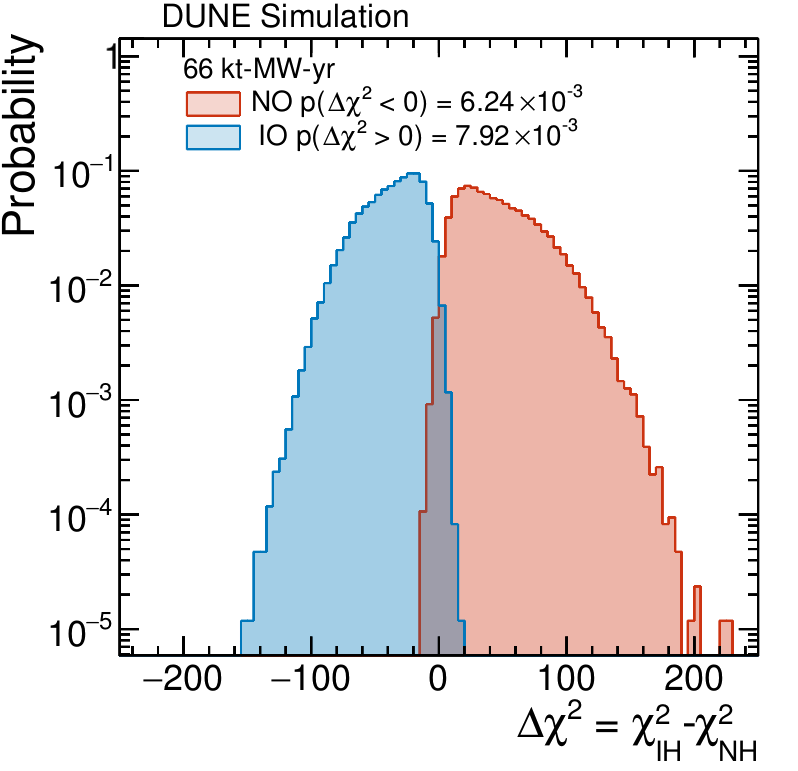
\includegraphics[width=0.33\linewidth]{MH_comp_ndfd_66ktMWyr_th13.png}}
  \subfloat[100 ktMWyr] {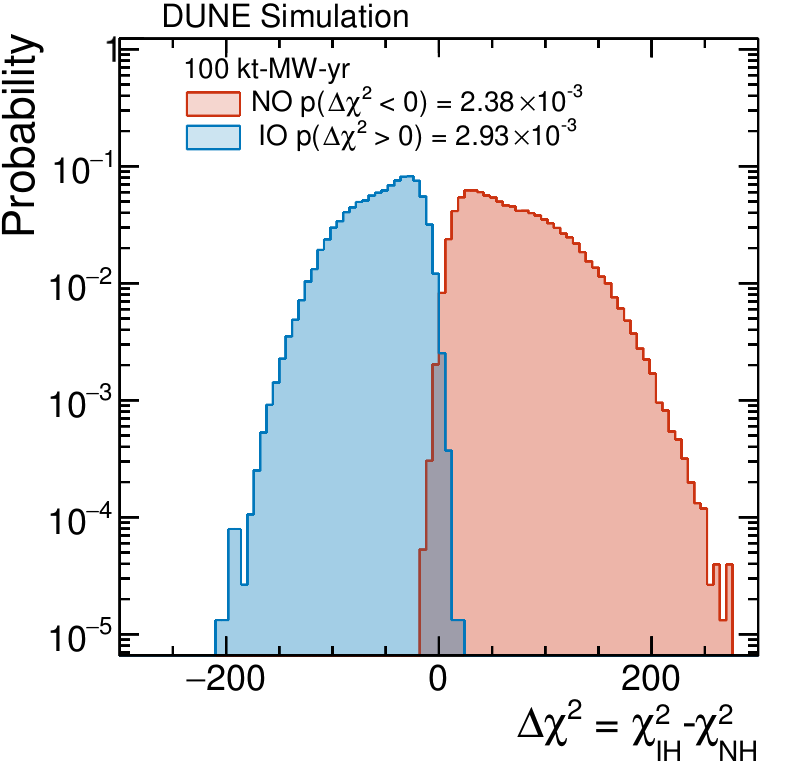
\includegraphics[width=0.33\linewidth]{MH_comp_ndfd_100ktMWyr_th13.png}}
  \subfloat[336 ktMWyr] {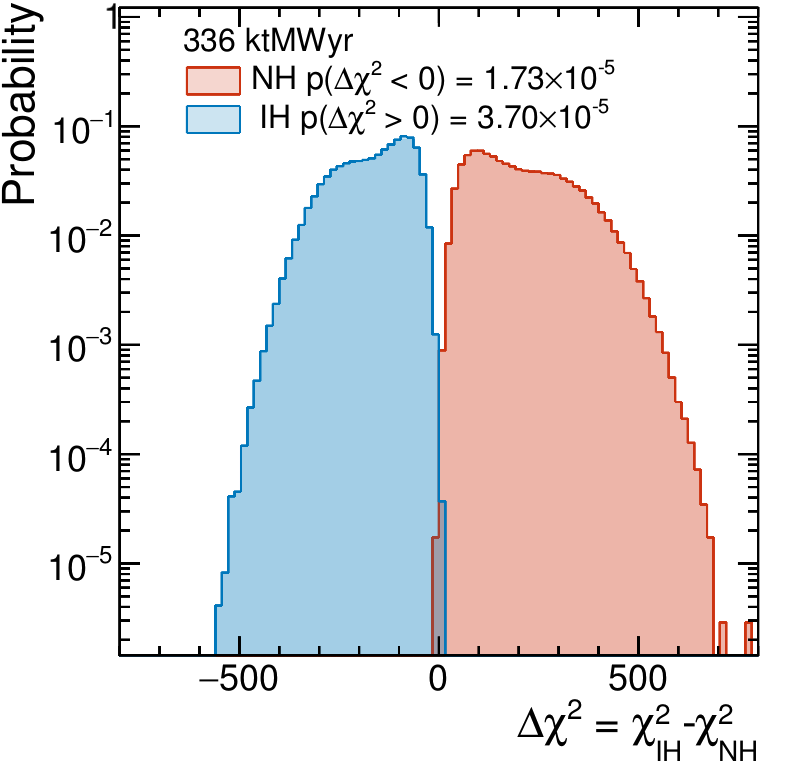
\includegraphics[width=0.33\linewidth]{MH_comp_ndfd_336ktMWyr_th13.png}}
  \caption{The distribution of $\dchisq = \chi^{2}_{\mathrm{IO}} - \chi^{2}_{\mathrm{NO}}$ values shown for both true normal (red) and true inverted (blue) hierarchies where . The fraction of throws for which the value of \dchisq is greater than (less than) 0 is also given for inverted (normal) hierarchies. For each ordering and exposure, approximately 100,000 throws were used.}
  \label{fig:mh_comp_over_time}
\end{figure*}
Given the complications with the interpretation of significance for mass ordering determination, it is instructive to look at the distribution of the test-statistic (Equation~\ref{eq:mh_chi2}), which gives more information than the 68\% central band and median throw shown in Figure~\ref{eq:mh_bands}. Figure~\ref{fig:mh_comp_over_time} shows the distribution of \dchisq obtained for a large ensemble of throws, for both true and inverted orderings, for a number of different exposures. Note that there is a uniform distribution of true \deltacp used in the throws. The separation between normal and inverted orderings shown increases over time, but the orderings are not degenerate even at very low exposures. The shape of the throw distribution is highly non-Gaussian, which makes it difficult to apply simple corrections to the sensitivity of the sort described in Ref.~\cite{Blennow:2013oma}. As a result we do not explore alternatives to $\sqrt{\dchisq}$ as a sensitivity metric, but note that the full information is given in Figure~\ref{fig:mh_comp_over_time}.

Figure~\ref{fig:mh_comp_over_time} also indicates the probability for the test statistic \dchisq to be less (more) than zero from the toy throws for true normal (inverted) hierarchies at each exposure. This marks the proportion of toys which appear more like the incorrect ordering than the true ordering for the toy. However, it is not easily converted to a single number sensitivity, although it does indicate the risk of a type I/type II error if the \dchisq value obtained by an experiment is exactly zero.

\begin{figure*}[htbp]
  \centering
  \subfloat[6 ktMWyr]   {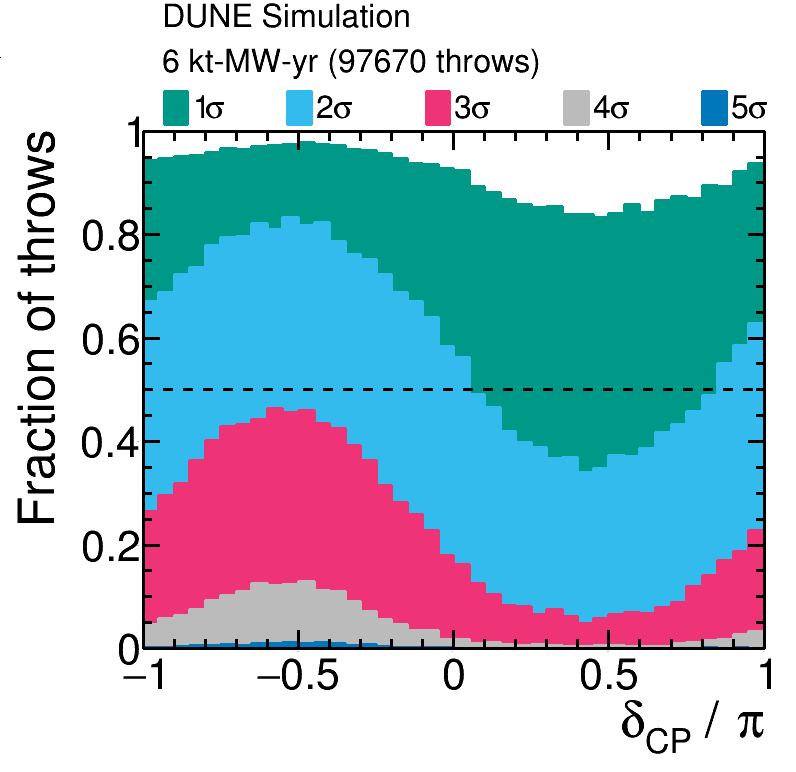
\includegraphics[width=0.33\linewidth]{mh_throws_6ktMWyr_NH_th13.png}}
  \subfloat[12 ktMWyr]  {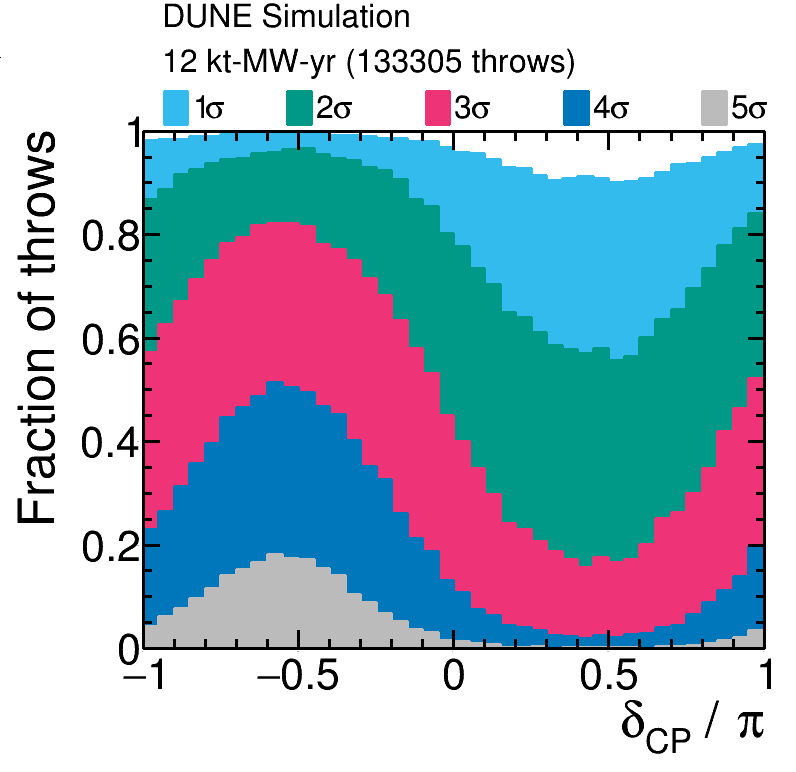
\includegraphics[width=0.33\linewidth]{mh_throws_12ktMWyr_NH_th13.png}}
  \subfloat[24 ktMWyr]  {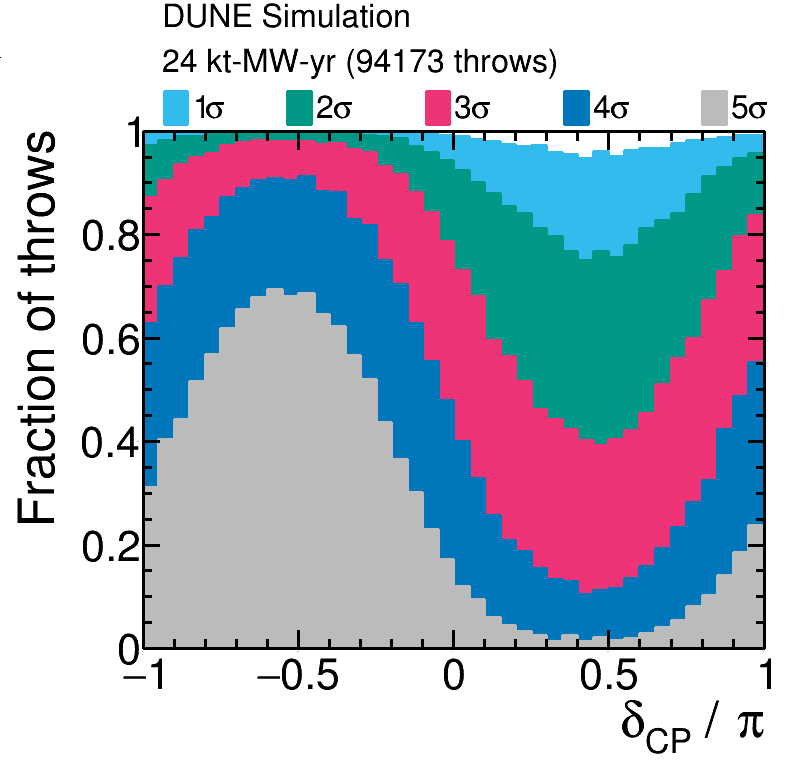
\includegraphics[width=0.33\linewidth]{mh_throws_24ktMWyr_NH_th13.png}}\\
  \subfloat[66 ktMWyr]  {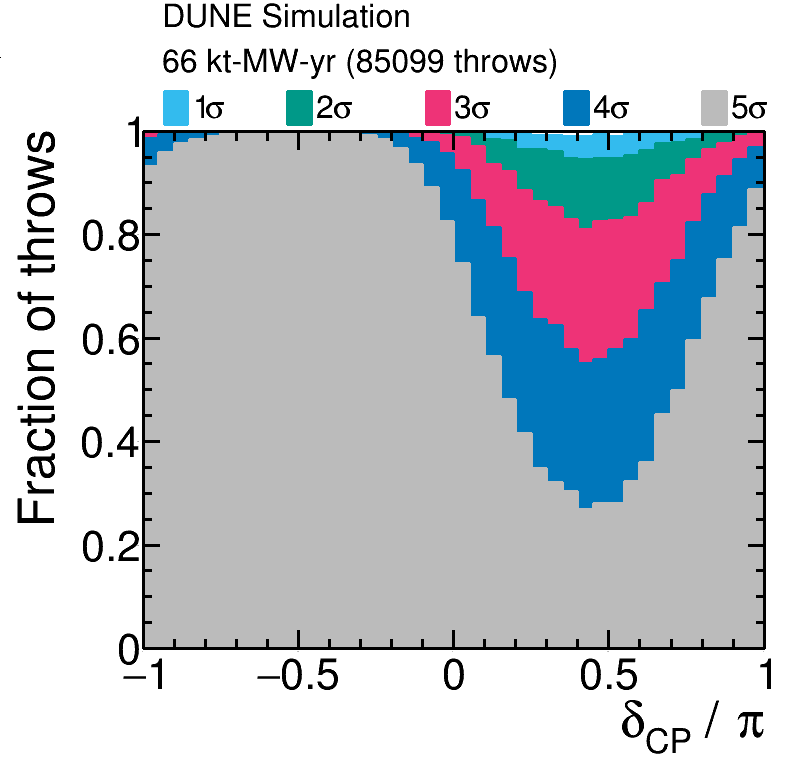
\includegraphics[width=0.33\linewidth]{mh_throws_66ktMWyr_NH_th13.png}}
  \subfloat[100 ktMWyr] {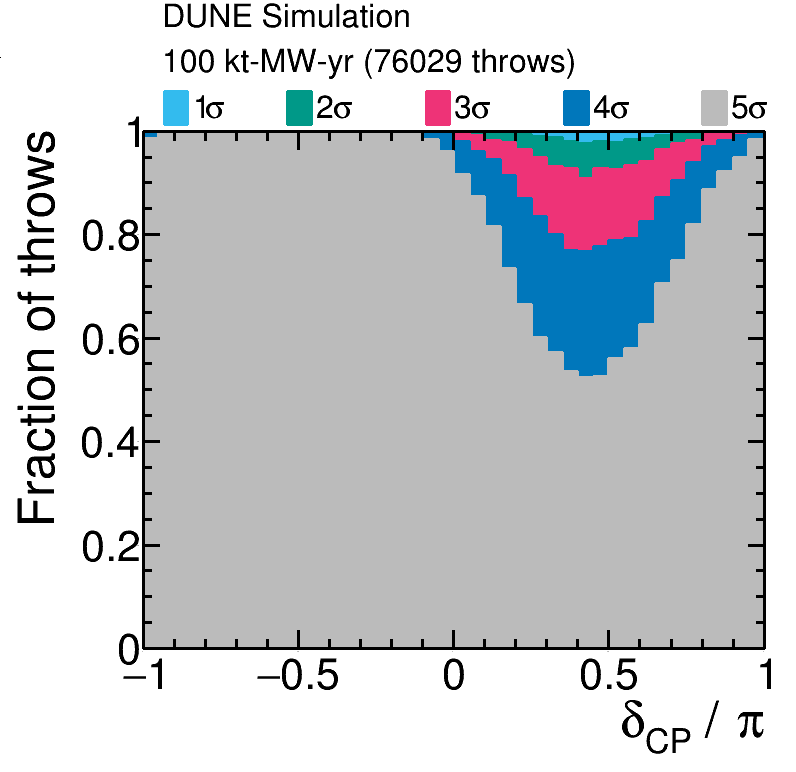
\includegraphics[width=0.33\linewidth]{mh_throws_100ktMWyr_NH_th13.png}}
  \subfloat[336 ktMWyr] {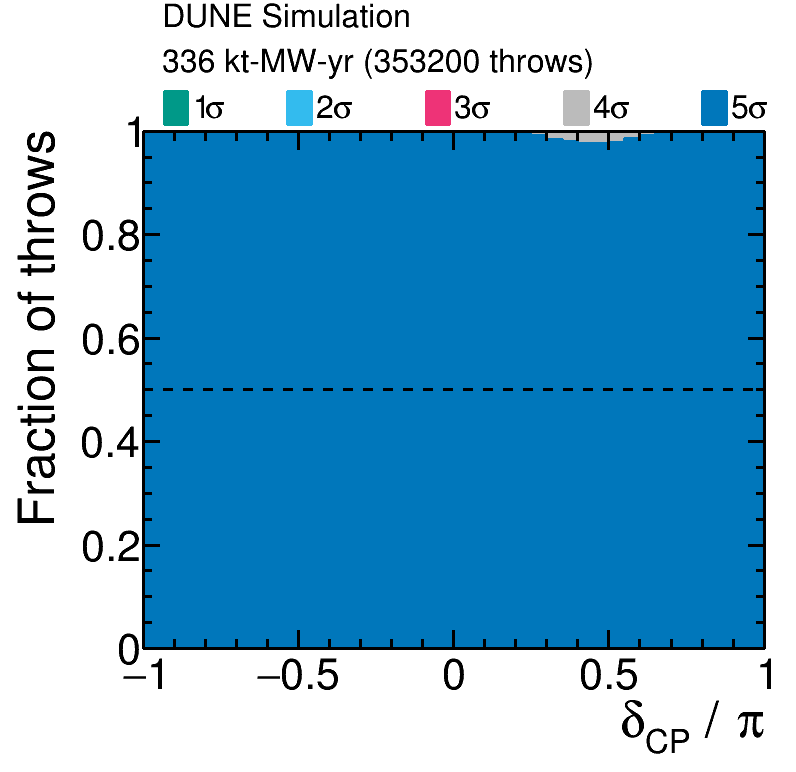
\includegraphics[width=0.33\linewidth]{mh_throws_336ktMWyr_NH_th13.png}}
  \caption{Fraction of throws for which the DUNE sensitivity to the mass ordering exceeds 1--5$\sigma$ significance, as a function of the true value of \deltacp. Shown for NO, for a number of different exposures. The number of throws used to make each figure is also shown.}
  \label{fig:mh_nh_over_time}
\end{figure*}

Figure~\ref{fig:mh_nh_over_time} shows the fraction of toy throws for which the \dchisq exceeds each significance threshold, for NO, shown as a function of \deltacp. The same throws are used as were used in Figures~\ref{fig:mh_comp_over_time} and~\ref{fig:mh_bands}. Despite the caveats regarding the intepretation of $\sqrt{\dchisq}$ as units of $\sigma$, the general trend is clear, and provides more information about the expected DUNE sensitivity at low exposures. As with Figure~\ref{fig:cpv_over_time}, the point at which the median sensitivity (50\% of throws) passes different significance thresholds can be easily read from the figures, and can be compared with those shown in Figure~\ref{fig:mh_bands}. The same general shape as a function of \deltacp as was observed in Figure~\ref{fig:mh_bands} can be seen. The general trend would be very similar in IO, reflected in the line $\deltacp = 0$. 
